\chapter{Classification of Comparative Sentences}
The data collected from the crowdsourcing task was used as training data for two classification problems. In the first problem, a machine learning algorithm was trained to predict one of the three classes per sentence (see table \ref{tbl:mainstudy-classes}). The second problem is a simplification of the first one as it is designed as a binary classification problem. The classes \texttt{BETTER} and \texttt{WORSE} were merged into the class \texttt{ARG}.

The data was split into a training set (5759 sentences; 4194 \texttt{NONE}, 1091 \texttt{BETTER} and 474 \texttt{WORSE}) and a held-out set.
The experiments were conducted on the training set only. During the development, the experiments were evaluated using stratified k-fold cross-validation where k equals five. 

The held-out set stayed untouched until the final evaluation presented in section \ref{sec:final}.

If not stated otherwise, scikit-learn (\cite{scikit-learn} was used to perform feature processing, the classification and evaluation.

\section{Choice of Algorithms}

\begin{figure}[htb]
\centering
\caption{F1 score of all tested classification algorithms. A binary bag-of-words feature was used as the baseline feature. Each algorithm was trained with five stratified folds of the data. The black bars show the standard derivation.}
\label{tbl:algo}
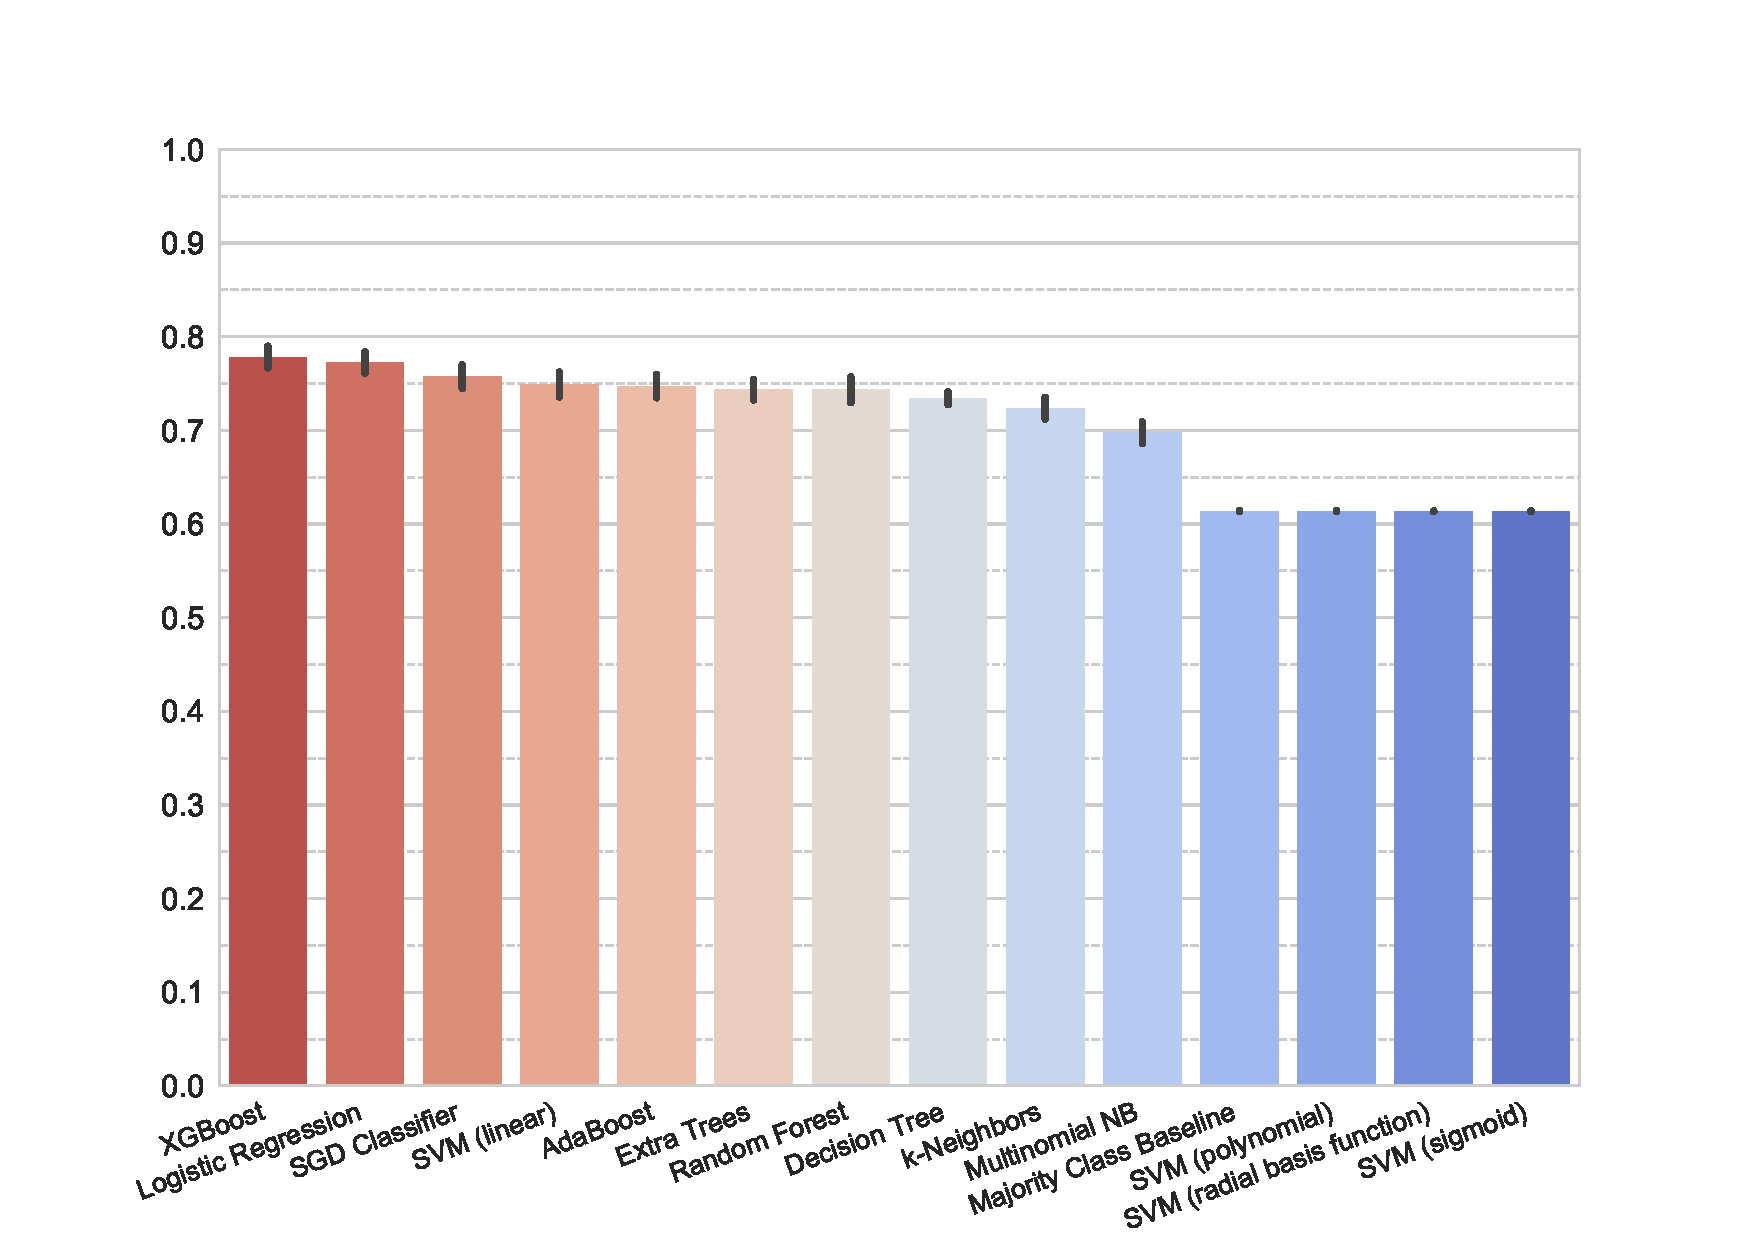
\includegraphics[width=0.8\linewidth]{images/classifier}
\end{figure}

To find the most suitable classification algorithms, thirteen (see figure \ref{tbl:algo}) were selected and compared. Except \emph{XGBoost}\footnote{XGBoost is not part of scikit-learn. The implementation presented in \cite{DBLP:journals/corr/ChenG16} was used.} and \emph{Extra Trees Classifier}, all algorithms were used in at least one paper presented in section \ref{sec:argmine}. A binary bag-of-words model computed on the whole sentence (see section \ref{sec:features}) was used as the sole feature. The f1 score was used as the metric to compare the algorithms. 

Tree-based methods and linear models worked good. Support Vector Machines with non-linear kernels assigned \texttt{NONE} to all sentences.

As XGBoost and Logistic Regression already work in a pleasing way, no further investigations on the performance of other algorithms was done. A set of hyper-parameters for XGBoost was tested using exhaustive grid search and randomized search. However, no significant increase in the f1 score could be achieved.

In the following sections, all experiments were conducted using XGBoost with 1000 estimators.


\section{Features}
\label{sec:features}
\subsection{Good title here}
Several vector representations were tested as features. The simplest one was a binary bag-of-words model realised with scikit-learns \texttt{CountVectorizer}. Another vector representation was generated with the five-hundred most frequent part-of-speech bi-, tri and four-grams. The mean word embedding vector was created by calculating the mean of each word's GloVe vector (as contained in spaCy's \texttt{en\_core\_web\_lg}\footnote{\url{https://spacy.io/models/en\#section-en\_core\_web\_lg}} model). Also, the pretrained InferSent model was used to create sentence embedding vectors.

A boolean feature capturing the appearance of a comparative adjective\footnote{Tag \emph{JJR} in the Penn Treebank (\url{https://www.ling.upenn.edu/courses/Fall\_2003/ling001/penn\_treebank\_pos.html})} was tested as well. Part-of-speech tagging for all features was done using spacy.\newline

Two preprocessing steps were used to generate the input for the feature calculation.

\begin{table}[ht]
\centering

\caption{Preprocessing examples for the sentence \enquote{\emph{In my mind, Python is better than Ruby}}}
\label{preprocessing_example}
\begin{tabularx}{\linewidth}{llX}
\toprule
Step 1 & Step 2 & Result \\ \midrule
Middle part & untouched & Python is better than Ruby \\
Middle part & removal & is better than \\
Full sentence & distinct replacement &In my mind, OBJECT\_A is better than OBJECT\_B \\
First part & removal & In my mind, \\
\bottomrule
\end{tabularx}

\end{table}

The first preprocessing step decided if the full sentence or a part of it should be used. The \emph{first part} contains all words from the beginning of the sentence to the first object, while the \emph{last part} contains all words from the second object to the end of the sentence. The \emph{middle part} contains all words between the first and the second object.

The second step was done to assess how important the objects are for the classification. The objects either stayed untouched, were removed or replaced. Two different replacement strategies were tested. First, both objects were replaced by the term \emph{OBJECT} (replacement). Second, the first object was replaced by \emph{OBJECT\_A} and the second by \emph{OBJECT\_B} (distinct replacement). This results in sixteen versions of each feature (four parts $\times$ four object strategies). Some examples are shown in table \ref{preprocessing_example}

\subsection{Dependency}
A feature based on LexNet was created to encode dependency information. The original code of LexNet was used to create the textual paths. It had to be modified, as the original code was to restrictive\footnote{The modified version is available at \url{https://github.com/ablx/LexNET}}. First, it allowed only paths up to a length of four edges. Second, it must be possible to reach the first object by following only left edges from the root, and the second object by following only right edges. The restrictions make sense for the original purpose of LexNet. However, XXXX sentences from the comparative argument mining data set do not get a path representation with those restrictions applied.



The neural network to encode the textual representations was implemented using Keras\footnote{\url{https://keras.io (Checked: 30.04.2018)}}, as presented in \cite{chollet2015keras}. The textual path representations were used to create target labels. The architecture is shown in figure \ref{fig:lexnetnn}.

\begin{figure}[h]
\centering
\caption{Architecture of the neural network used to encode textual dependency paths to vectors.}
\label{fig:lexnetnn}
\end{figure}





\section{Experiments}
\subsection{Baselines}
\label{sec:3_baseline}
As described in section \ref{sec:argmine}, there is no task which is similar enough the one at hand which could be used as a baseline. Thus, two baselines using the obtained data were created. The first baseline, shown in table \ref{tbl:3stratifiedbaseline} and \ref{tbl:binmaj}, assigns all sentences to the class \texttt{NONE}.

% 24.3
\begin{table}[!htb]
	\begin{minipage}{.5\linewidth}
		\caption{Random (stratified) baseline for the three-label scenario.}
		\label{tbl:3stratifiedbaseline}
		\centering
		      
		\begin{tabularx}{0.97\linewidth}{Xrrrr}
			\toprule
			                & precision                    & recall                       & f1 score                     \\ \midrule 
			\texttt{BETTER} & 0.22 \scriptsize{$\pm$0.02} & 0.23 \scriptsize{$\pm$0.02} & 0.22 \scriptsize{$\pm$0.02} \\ 
			\texttt{WORSE}  & 0.10 \scriptsize{$\pm$0.02} & 0.08 \scriptsize{$\pm$0.02} & 0.09 \scriptsize{$\pm$0.02} \\ 
			\texttt{NONE}   & 0.74 \scriptsize{$\pm$0.00}  & 0.74 \scriptsize{$\pm$0.01} & 0.74 \scriptsize{$\pm$0.01} \\ 
			avg.         & 0.59 \scriptsize{$\pm$0.01} & 0.59 \scriptsize{$\pm$0.01} & 0.59 \scriptsize{$\pm$0.01} \\ 
			\bottomrule
		\end{tabularx} 
		
	\end{minipage}%
	\begin{minipage}{.5\linewidth}
		\centering
		\caption{Majority class baseline for the  for the three-label scenario.}
		\label{tbl:3majoritybaseline}
		\begin{tabularx}{0.97\linewidth}{Xrrrr}
			\toprule
			                & precision                    & recall                       & f1 score                                    \\ \midrule 
			\texttt{BETTER} & 0.00 \scriptsize{$\pm$0.00} & 0.00 \scriptsize{$\pm$0.00} & 0.00 \scriptsize{$\pm$0.00}                \\ 
			\texttt{WORSE}  & 0.00 \scriptsize{$\pm$0.00} & 0.00 \scriptsize{$\pm$0.00} & 0.00 \scriptsize{$\pm$0.00}                \\ 
			\texttt{NONE}   & 0.73 \scriptsize{$\pm$0.00}     & 1.00 \scriptsize{$\pm$0.00} & 0.84 \scriptsize{$\pm$0.00}                \\ 
			avg.         & 0.53 \scriptsize{$\pm$0.00} & 0.73 \scriptsize{$\pm$0.00} & \textbf{0.61} \scriptsize{$\pm$0.00} \\ 
			\bottomrule
		\end{tabularx}
	\end{minipage} 
\end{table}


The second baseline was created by assigning classes to the data at random, respecting the distribution of classes in the original data. The results are shown in tables \ref{tbl:3majoritybaseline} and \ref{tbl:binstrat}.



\begin{table}[!htb]
	\begin{minipage}{.5\linewidth}
		\caption{Random (stratified) baseline for the binary scenario.}
		\label{tbl:binmaj}
		\centering
		      
		\begin{tabularx}{0.97\linewidth}{Xrrrr}
			\toprule
			              & precision                    & recall                       & f1 score                              \\ \midrule 
			\texttt{ARG}  & 0.31 \scriptsize{$\pm$0.02} & 0.31 \scriptsize{$\pm$0.02} & 0.31 \scriptsize{$\pm$0.02}          \\ 
			\texttt{NONE} & 0.74 \scriptsize{$\pm$0.01} & 0.74 \scriptsize{$\pm$0.01} & 0.74 \scriptsize{$\pm$0.01}          \\ 
			avg.       & 0.62 \scriptsize{$\pm$0.01} & 0.62 \scriptsize{$\pm$0.01} & \textbf{0.62} \scriptsize{$\pm$0.01} \\ 
			\bottomrule
		\end{tabularx}
		
	\end{minipage}%
	\begin{minipage}{.5\linewidth}
		\centering
		\caption{Majority class baseline for the binary scenario.}
		\label{tbl:binstrat}
		\begin{tabularx}{0.97\linewidth}{Xrrrr}
			\toprule
			              & precision                    & recall                       & f1 score                     \\ \midrule 
			\texttt{ARG}  & 0.00 \scriptsize{$\pm$0.00} & 0.00 \scriptsize{$\pm$0.00} & 0.00 \scriptsize{$\pm$0.00} \\ 
			\texttt{NONE} & 0.73 \scriptsize{$\pm$0.00} & 1.00 \scriptsize{$\pm$0.00} & 0.84 \scriptsize{$\pm$0.00} \\ 
			avg.       & 0.53 \scriptsize{$\pm$0.00} & 0.73 \scriptsize{$\pm$0.00} & 0.61 \scriptsize{$\pm$0.00} \\ 
			\bottomrule
		\end{tabularx}
	\end{minipage} 
\end{table}
For all baselines, the scikit-learn's \texttt{DummyClassifer} was used.

\subsection{Results}
\label{sec:3_results}
The classification results for the best performing feature configurations in the three-class scenario are presented in figures \ref{fig:3_f1} (f1 score), \ref{fig:3_precision} (precision) and \ref{fig:3_recall} (recall). Each feature was tested and evaluated using five stratified folds. Presented are the overall results and the results for each class. The black bar shows the standard derivation. All scores were calulcated with scikit-learn's metric module (\texttt{sklearn.metrics}). All features use the middle part of the sentence and left the objects untouched.


\begin{figure}[h]
      \caption{\textbf{F1 score} for the three-class scenario using XGBoost. The blue bar shows the weighted average of each class. The feature name (see section \ref{sec:features}) is presented on the x-axis, the f1 score on the y-axis. The black bar displays the standard derivation.} 
    \label{fig:3_f1}
 \centering
	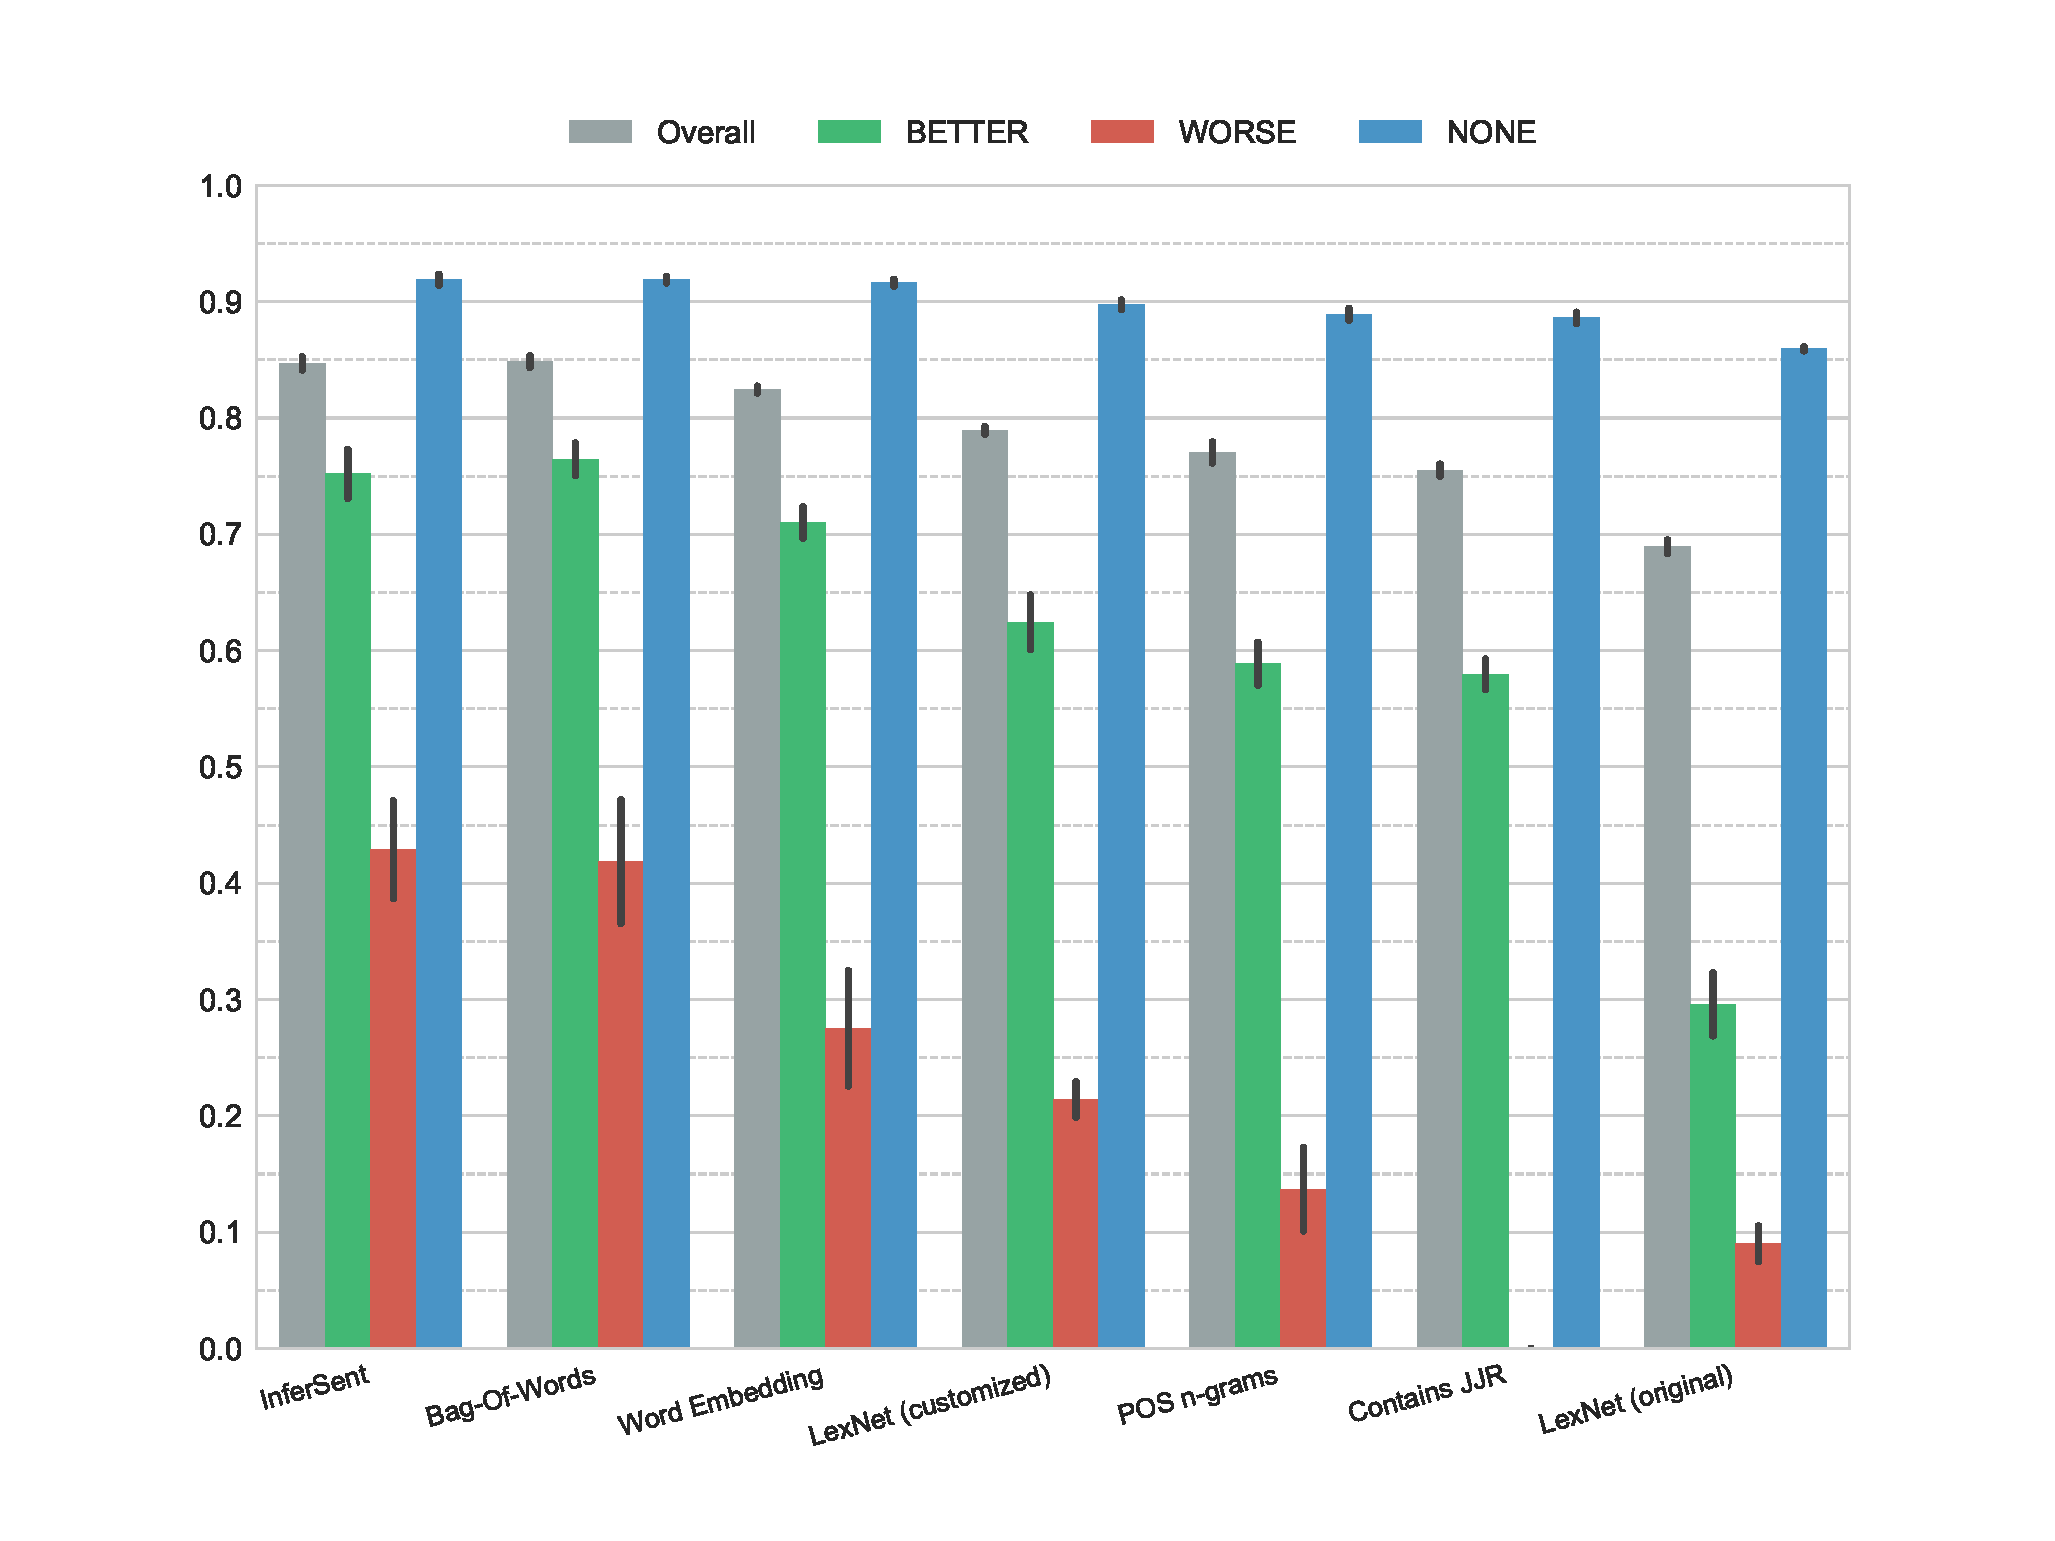
\includegraphics[width=0.9\textwidth]{images/experiments/f1-False}

\end{figure}

All features yield f1 scores at least fifteen points over the baseline. Bag-of-words (f1 score 0.855) and InferSent (f1 score 0.858) deliver almost identical results. The boolean feature that captures comparative adjectives in the middle of the sentence yields a f1 score over the baseline as well. However, it does not assign any examples to the class \texttt{WORSE}.



% === binary 
Figures \ref{fig:2_f1} (f1 score), \ref{fig:2_precision} (precision) and \ref{fig:2_recall} (recall) show the results for the binary classification.
\begin{figure}[h]
      \caption{\textbf{F1 score} for the binary scenario using XGBoost. The blue bar shows the weighted average of each class. The feature name (see section \ref{sec:features}) is presented on the x-axis, the f1 score on the y-axis. The black bar displays the standard derivation.} 
    \label{fig:3_f1}

    \label{fig:2_f1}
 \centering
	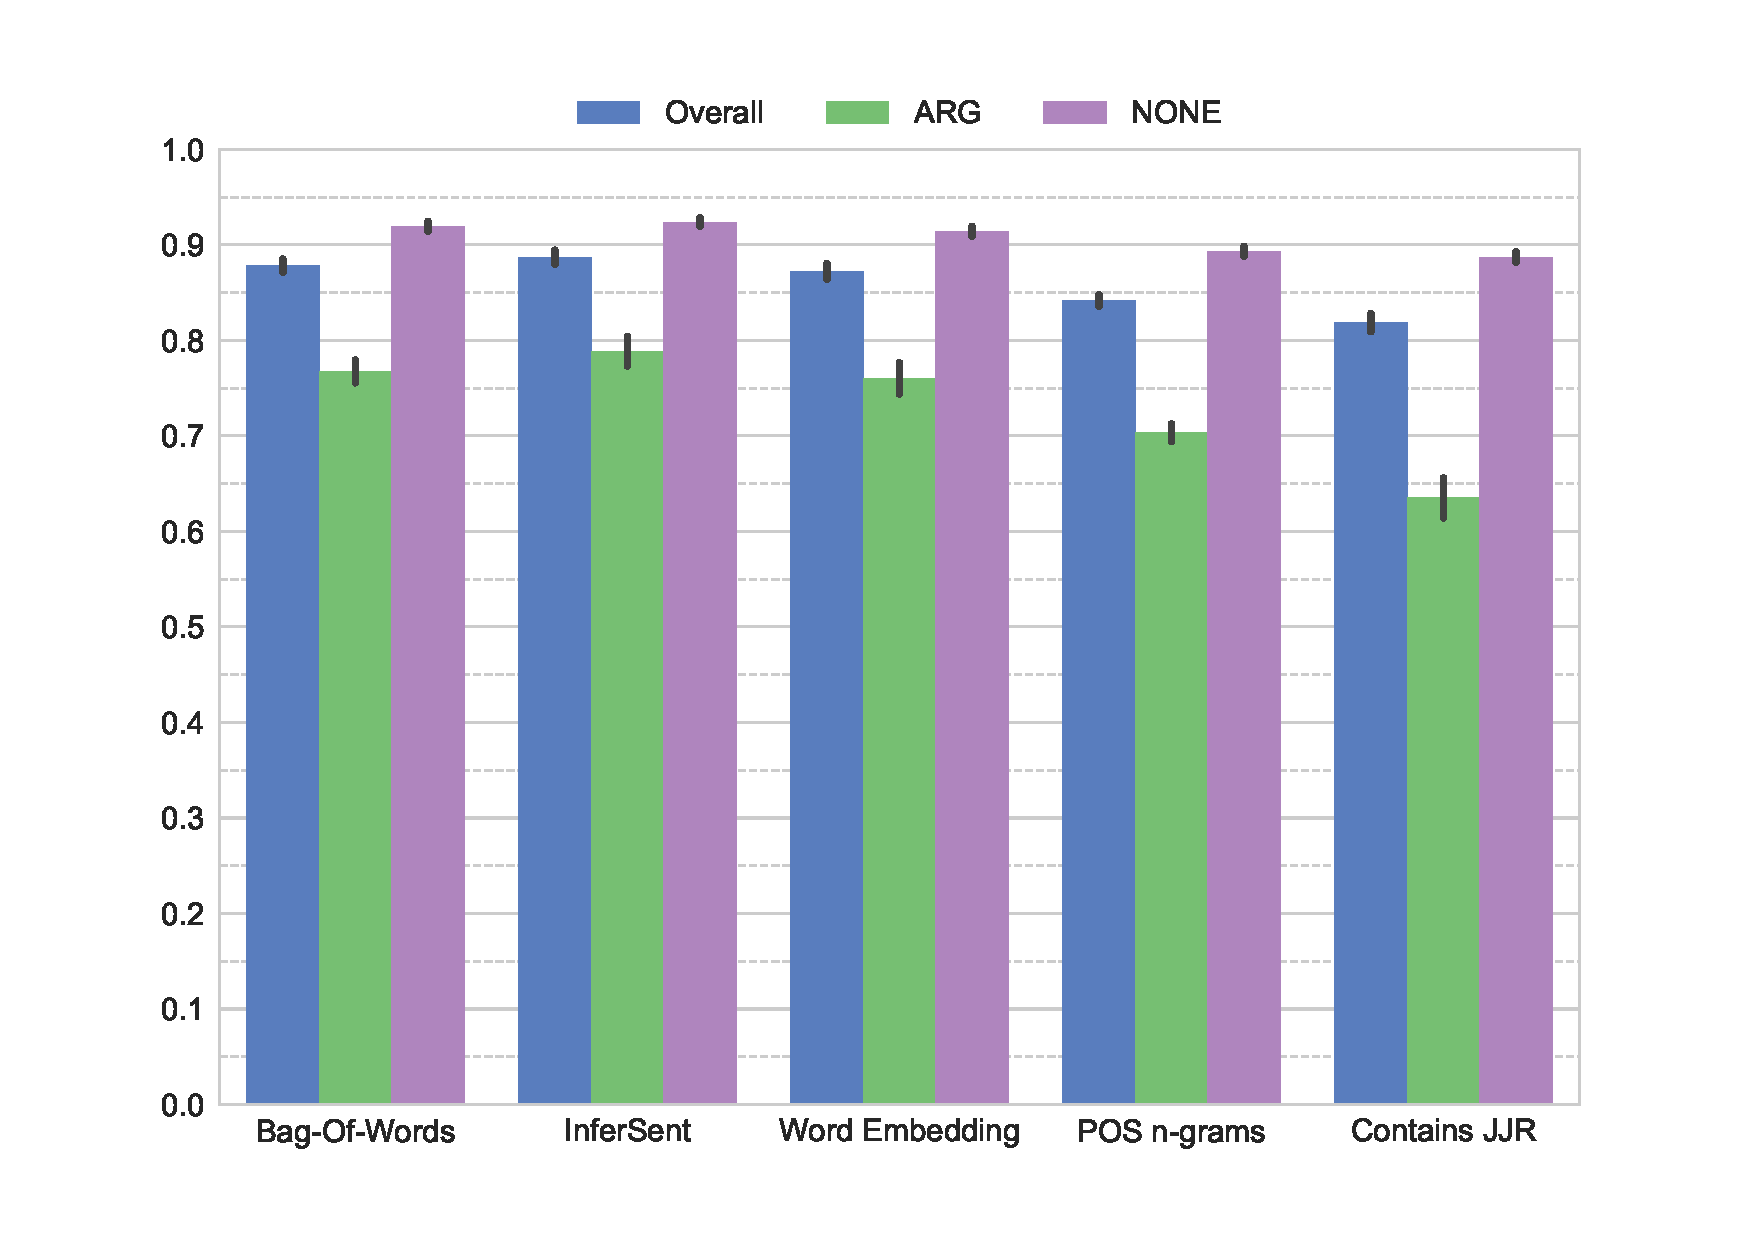
\includegraphics[width=0.9\textwidth]{images/experiments/f1-True}

\end{figure}
As with the three-class scenario, InferSent (f1 score 0.894) and the bag-of-words (f1 score 0.890) performed best and got almost equal results. In contrast to the three-classes scenario, they are closely followed by mean word embeddings. In summary, all vector representations worked good and got f1 scores close to each other. The feature capturing the appearance of comparative adjectives is again the worst, yet the score is nineteen points above the baseline.



\begin{figure}[tb]
         \caption{\textbf{Precision} for the three-class scenario using XGBoost. The blue bar shows the weighted average of each class. The feature name (see section \ref{sec:features}) is presented on the x-axis, the precision score on the y-axis. The black bar displays the standard derivation.} 
    \label{fig:3_precision}
 \centering
	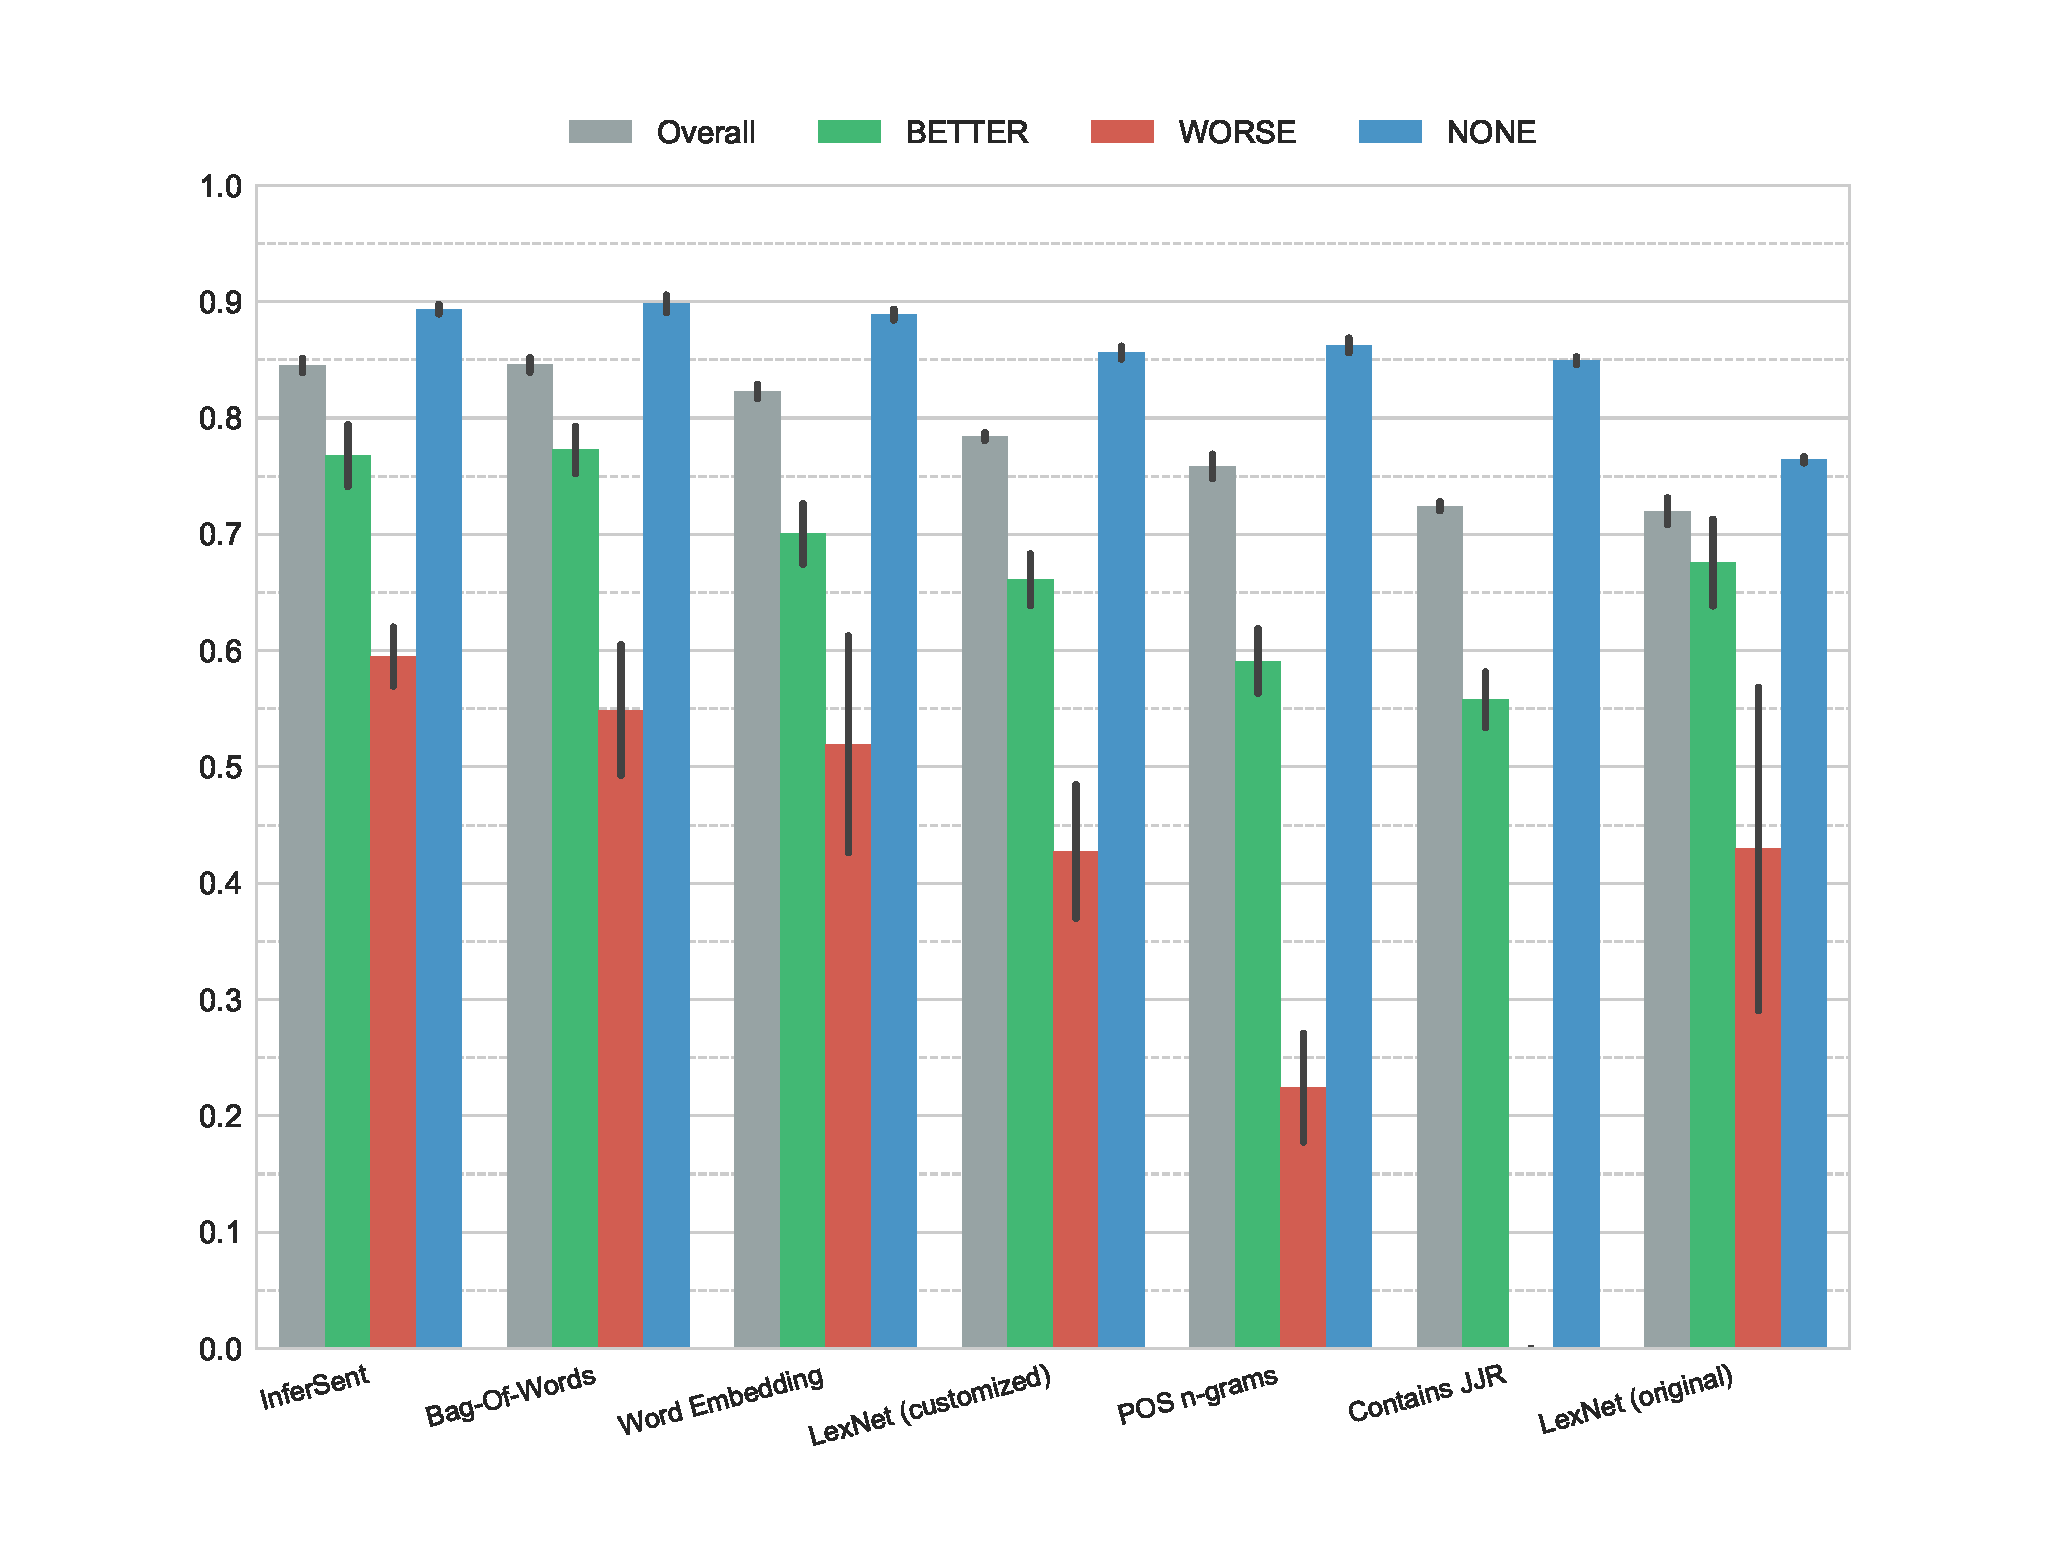
\includegraphics[width=0.9\textwidth]{images/experiments/precision-False}
\end{figure}

  \begin{figure}[p]
              \caption{\textbf{Recall} for the three-class scenario using XGBoost. The blue bar shows the weighted average of each class. The feature name (see section \ref{sec:features}) is presented on the x-axis, the recall score on the y-axis. The black bar displays the standard derivation.} 
       \label{fig:3_recall}
 \centering
	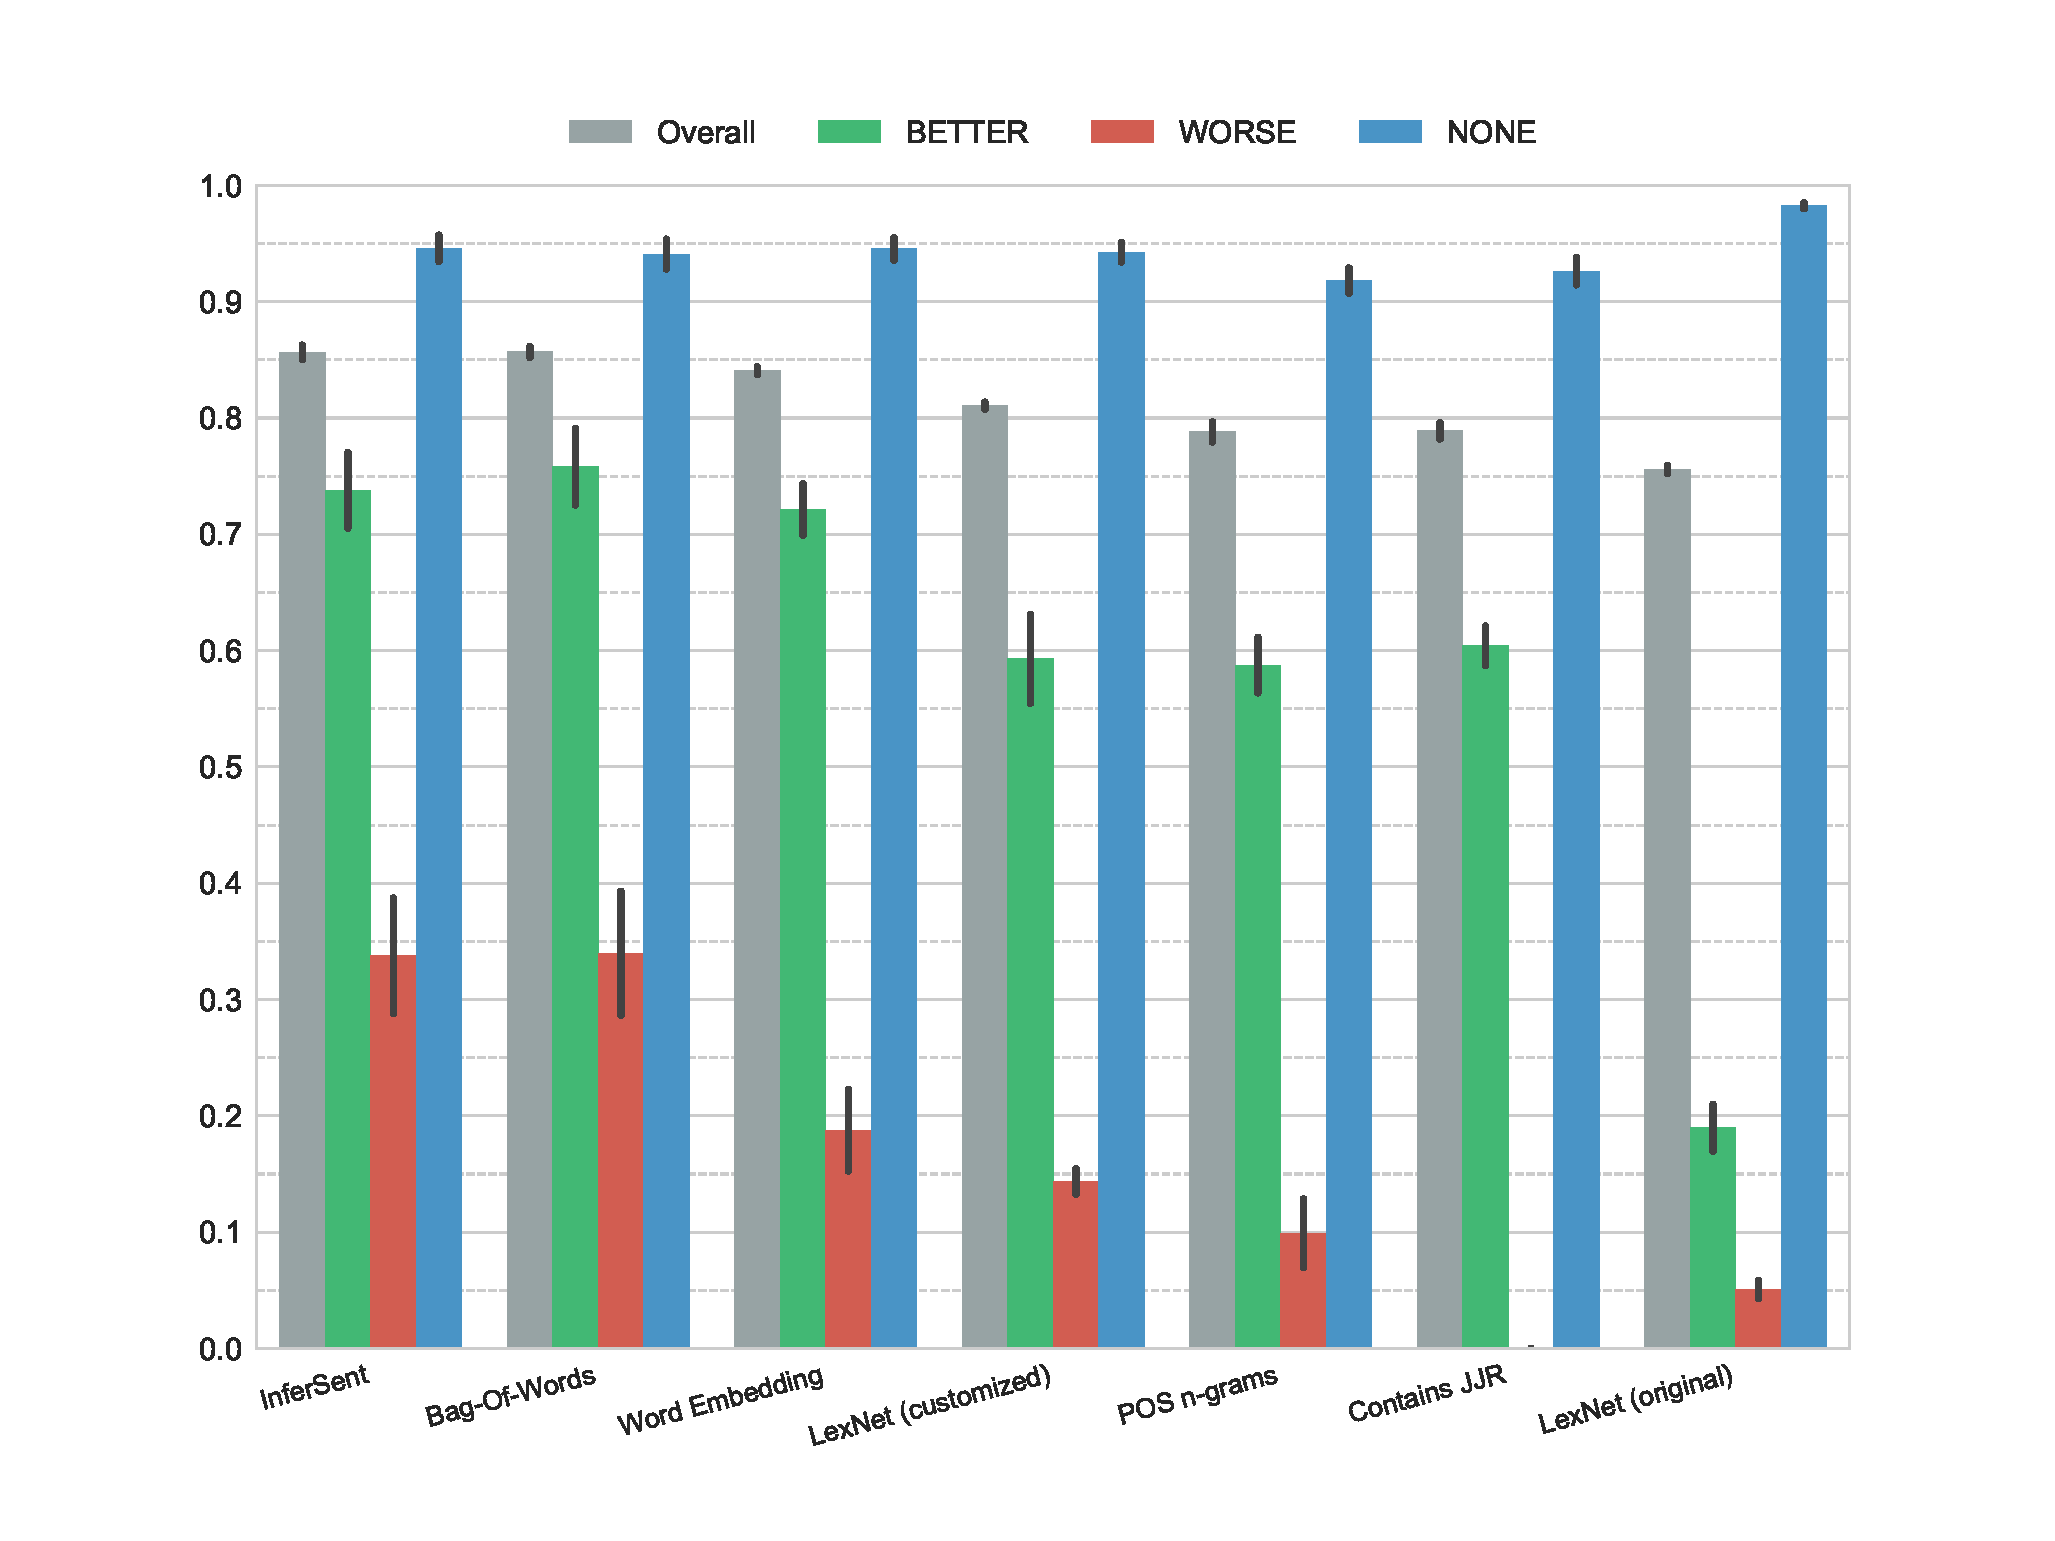
\includegraphics[width=1\textwidth]{images/experiments/recall-False}
\end{figure}



\begin{figure}[tb]
         \caption{\textbf{Precision} for the binary scenario using XGBoost. The blue bar shows the weighted average of each class. The feature name (see section \ref{sec:features}) is presented on the x-axis, the precision score on the y-axis. The black bar displays the standard derivation.} 
    \label{fig:2_precision}
    \centering
	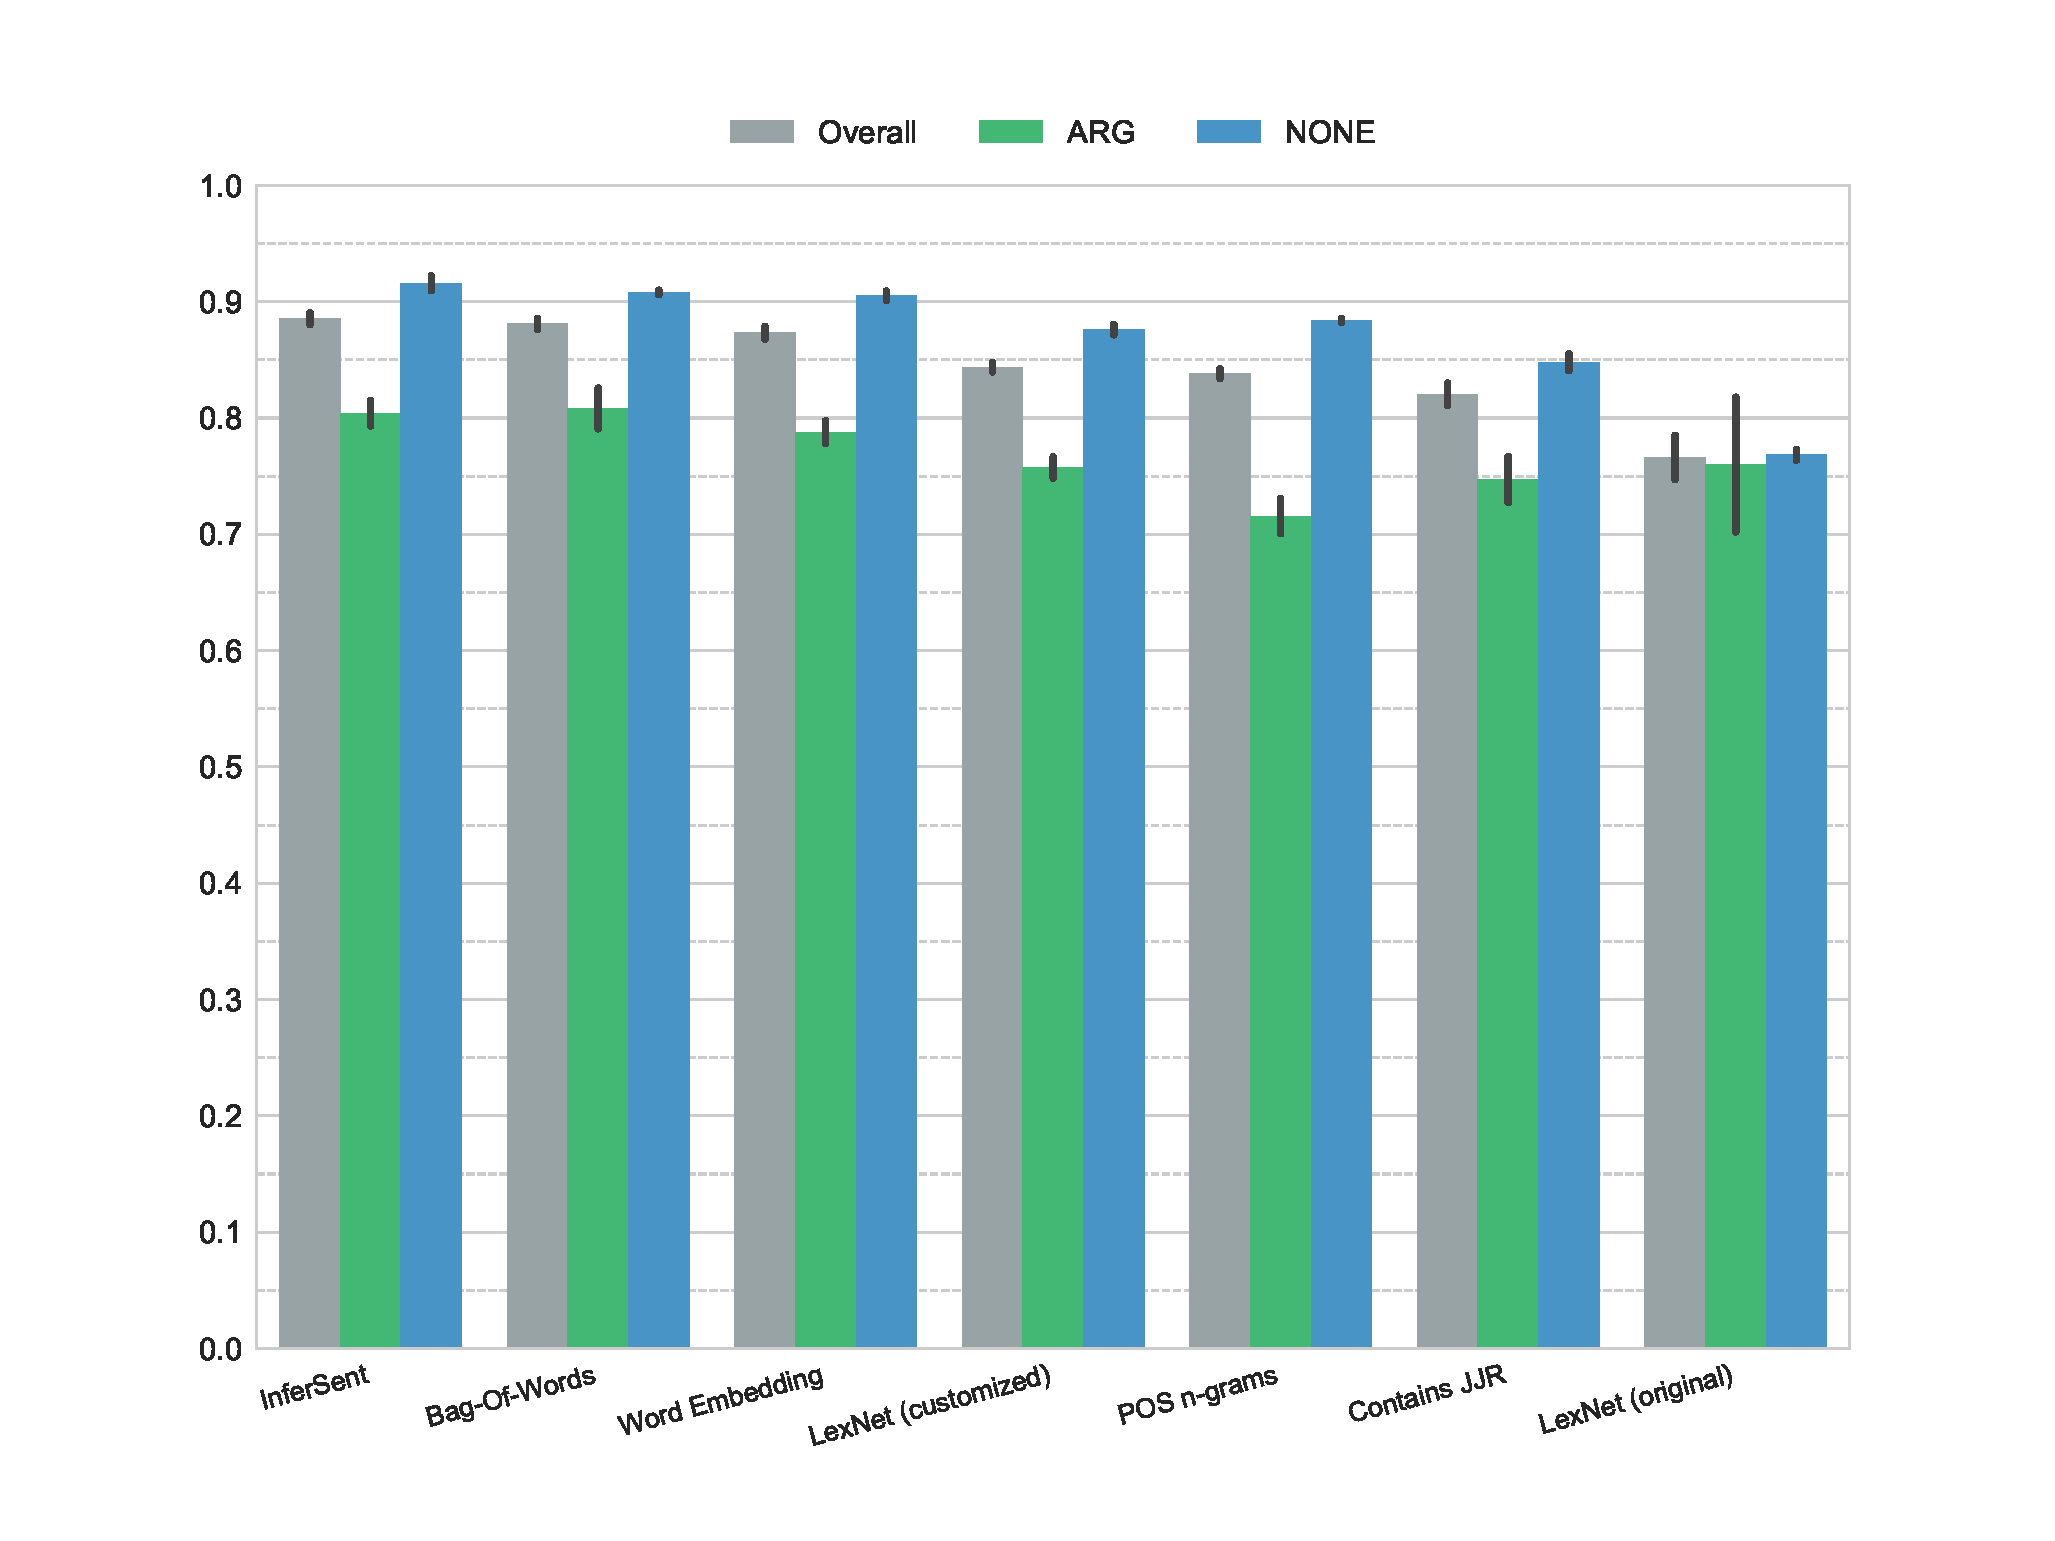
\includegraphics[width=0.9\linewidth]{images/experiments/precision-True}
    \end{figure}
    
    \begin{figure}[tb]
              \caption{\textbf{Precision} for the binary scenario using XGBoost. The blue bar shows the weighted average of each class. The feature name (see section \ref{sec:features}) is presented on the x-axis, the binary score on the y-axis. The black bar displays the standard derivation.} 
       \label{fig:2_recall}
 \centering
	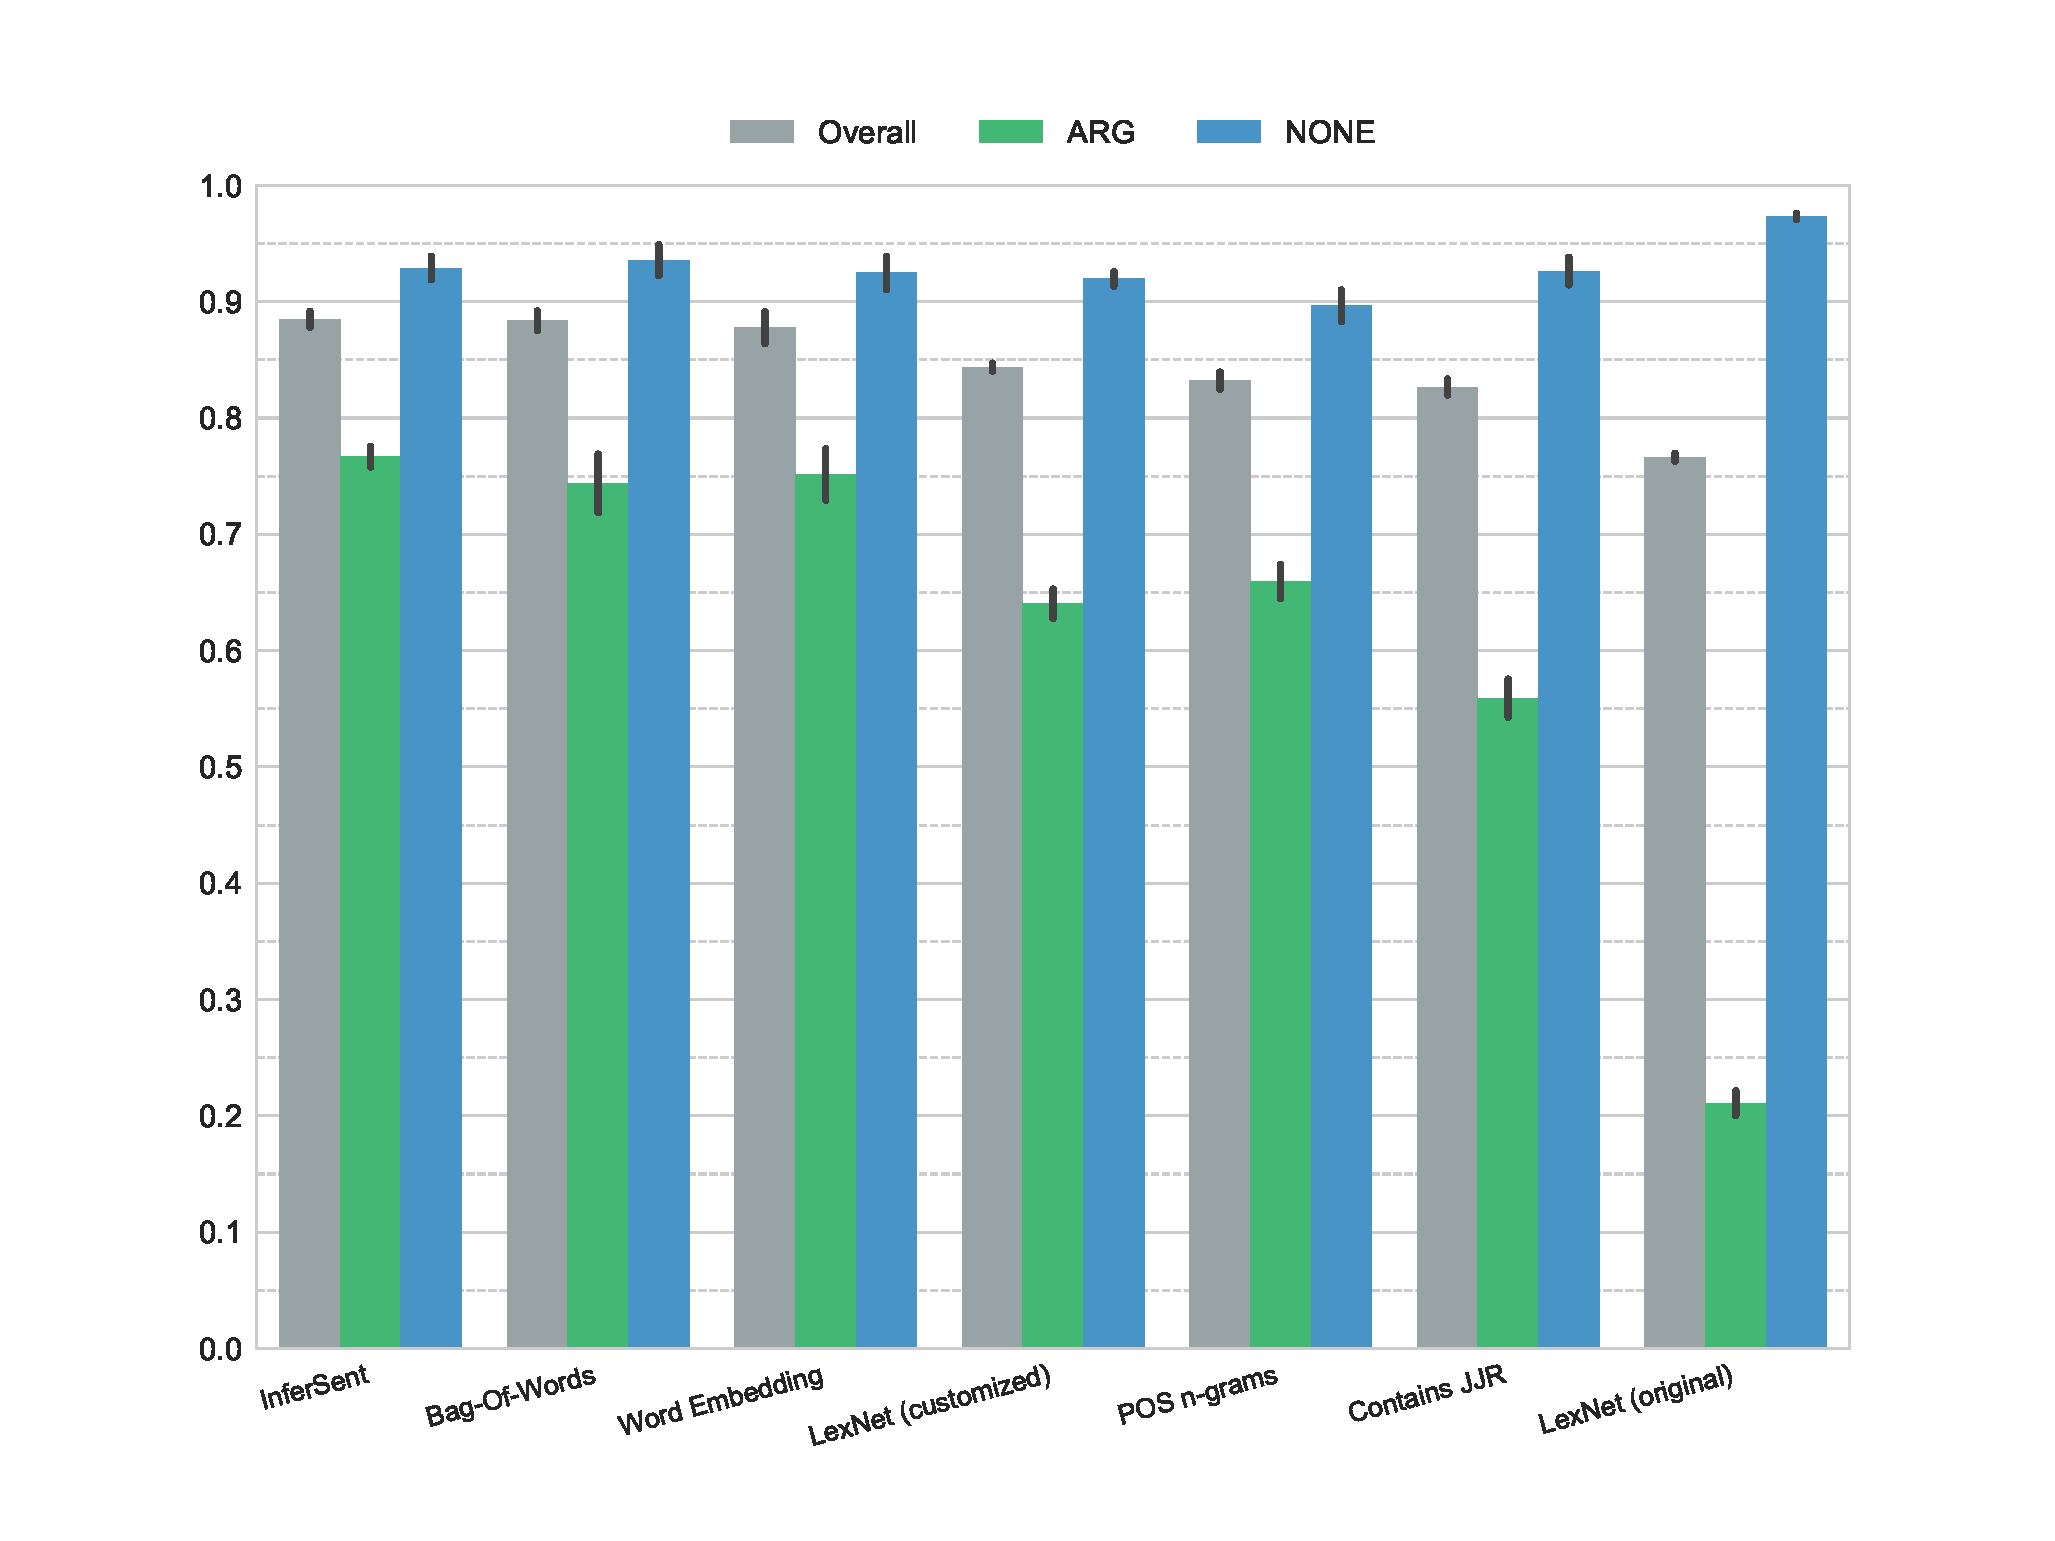
\includegraphics[width=0.9\linewidth]{images/experiments/recall-True}

\end{figure}



\FloatBarrier
\subsection{Error analysis}
\label{sec:error_analysis}
Figures \ref{fig:3_conf_inf} and \ref{fig:3_conf_uni} display the confusion matrices for the two best features in the three-label scenario (InferSent and bag-of-words). The confusion matrices of each fold per feature were summed up to create these tables.





\begin{figure}[h]
    \begin{minipage}{.5\linewidth}
   \caption{Confusion matrix for the InferSent feature using XGBoost} 
    \label{fig:3_conf_inf}
 \centering
	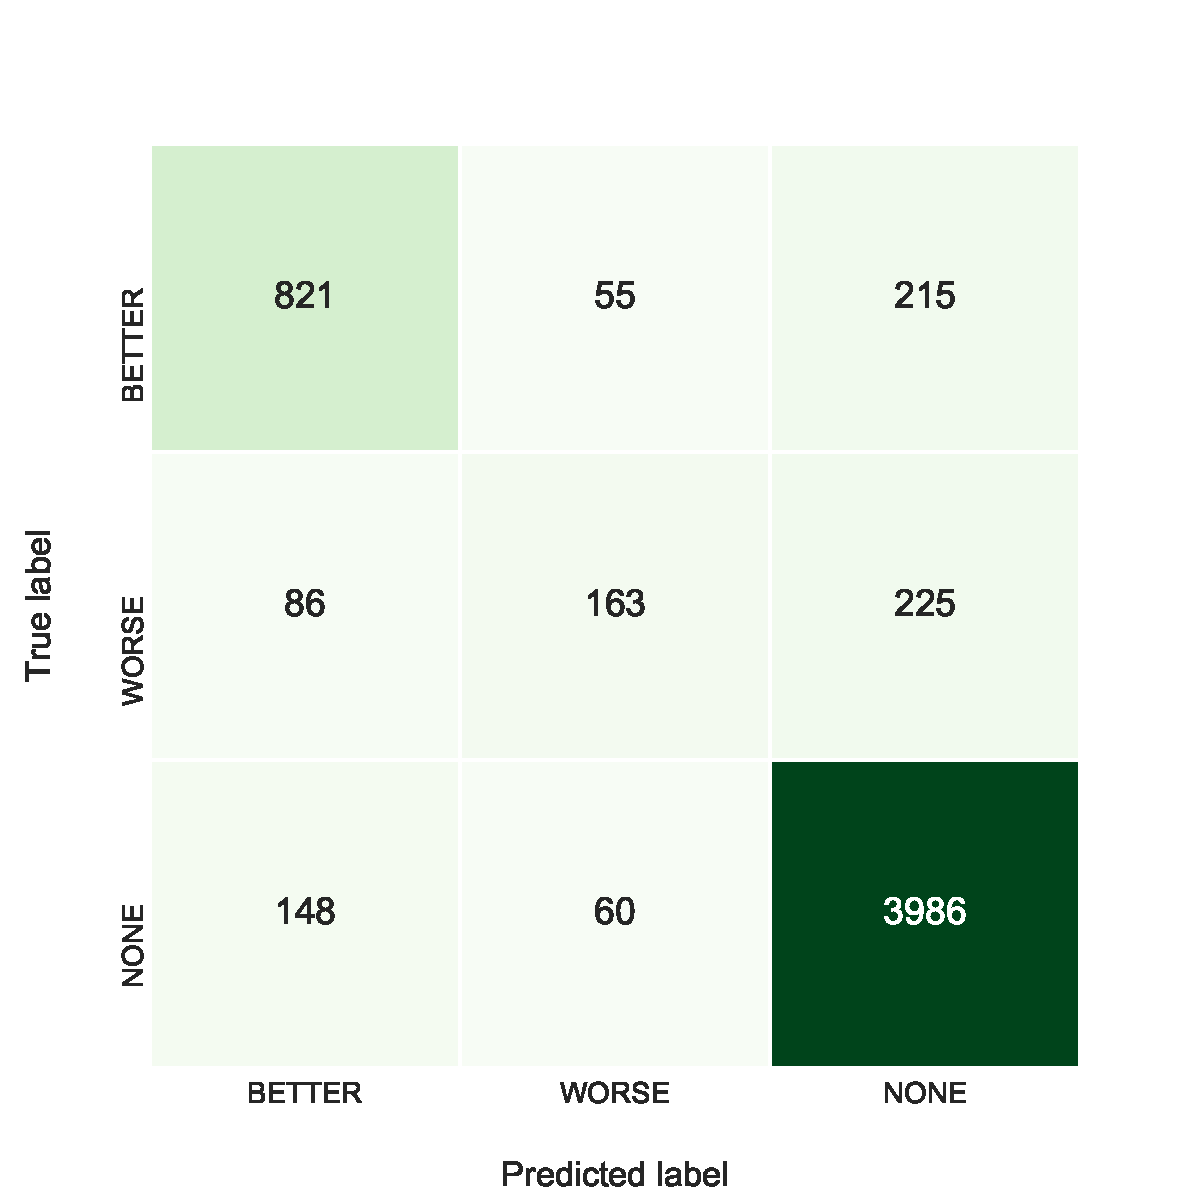
\includegraphics[width=1\linewidth]{images/experiments/conf-InferSent_False}
  \end{minipage} \hfill
    \begin{minipage}{.5\linewidth}
  
     \caption{Confusion matrix for the bag-of-words feature using XGBoost} 
       \label{fig:3_conf_uni}
 \centering
	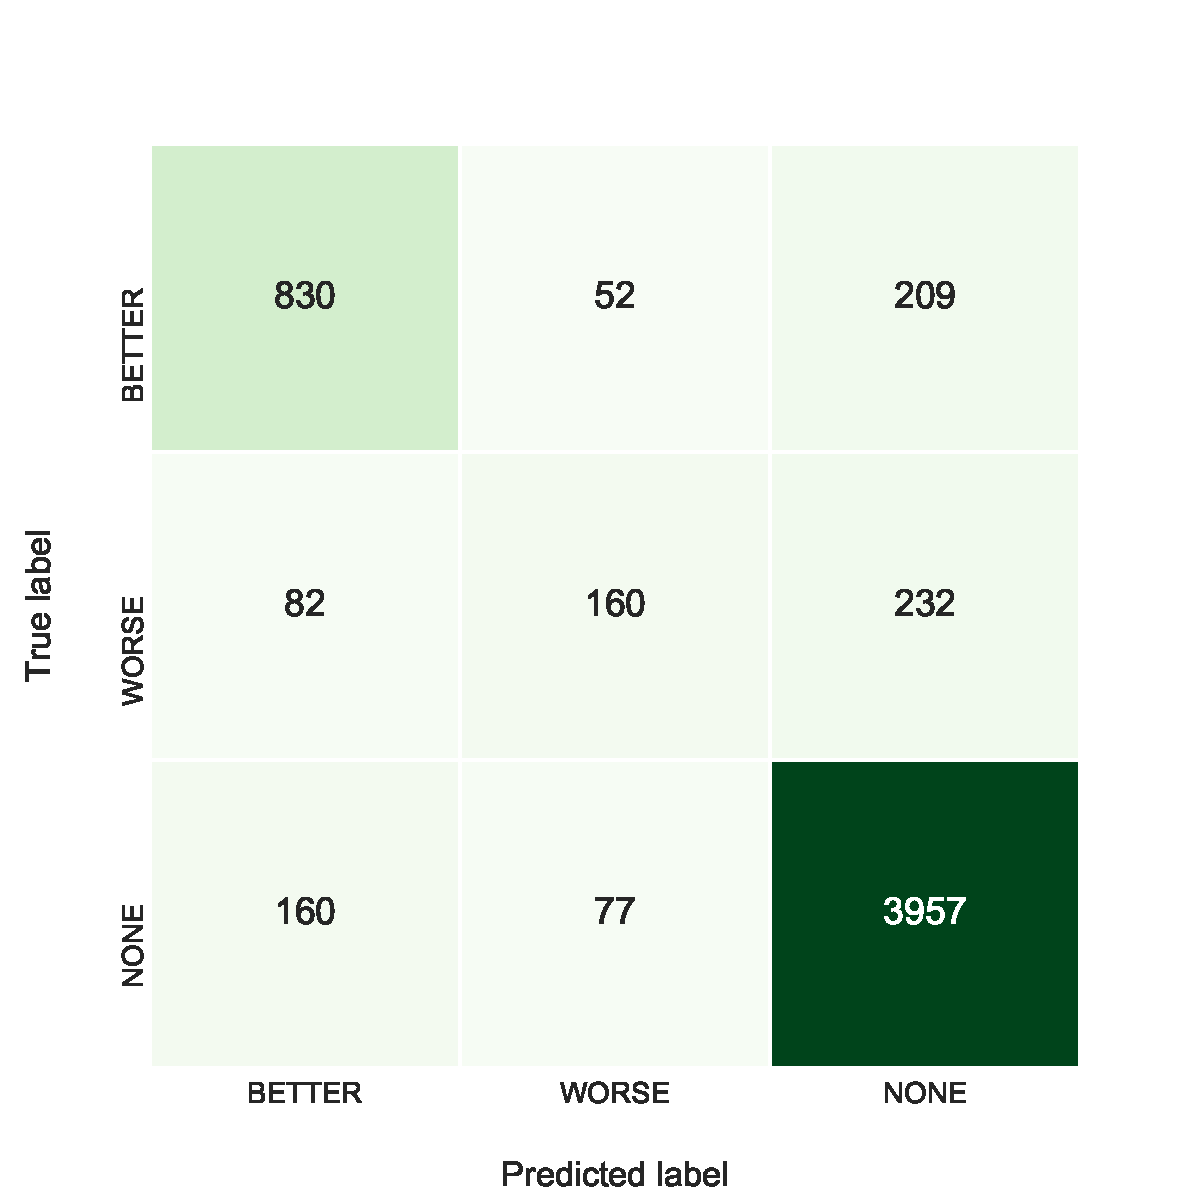
\includegraphics[width=1\linewidth]{images/experiments/conf-Bag-Of-Words_False}
    \end{minipage} 
\end{figure}

As presented above, \texttt{WORSE} was the hardest class to recognize. The matrices show that it was more often confused with \texttt{NONE} than with \texttt{BETTER}. This is contrary to the expections. \texttt{BETTER} and \texttt{WORSE} both represent argumentative sentences and it was expected that the distinction between argumentative and not-argumentative is clearer. 

Both features made the same errors on 661 sentences. The unigram model made another 174 errors on sentences which were correctly predicted by the sentence embedding model. The sentence embedding model made 164 unique errors. However, there is no clear pattern which sentences are hard for the unigram or sentence embedding feature. One-hundred-and-fifty wrongly predicted sentences were analysed, examples are shown in table \ref{tbl:3_mistakes}. 

\begin{table}[h]
\caption{Example sentences for errors made by the classifier in the three-label scenario. The objects of interest are printed \textbf{bold}, the assumed error source in \emph{italics}. Confidence shows the confiedence of the annotators and is calculated as \emph{judgments for majority class / total judgments}.}
\label{tbl:3_mistakes}
\begin{tabularx}{\linewidth}{Xrrr}
\toprule
 Sentence & Predicted & Gold & Confidence \\ \midrule
 Is a \textbf{BMW}/Benz 5x better than a \textbf{Honda} Civic\emph{?} & \texttt{BETTER} & \texttt{NONE} & 0.6 \\
 Will \textbf{google} Music Become Bigger and Better than \textbf{itunes}\emph{?}& \texttt{BETTER} & \texttt{NONE} & 0.5 \\

Apparently the \textbf{wii} \emph{isn't} superior to the \textbf{ds} for Square-enix. & \texttt{BETTER} & \texttt{WORSE} & 0.8 \\
 We usually \emph{don't} like \textbf{Microsoft}, but I \emph{don't} think they are worse than \textbf{Google}. & \texttt{WORSE} & \texttt{BETTER} & 0.6 \\

 \emph{Worse} than \textbf{coffee}, the effect \textbf{beer} has on my bladder. & \texttt{NONE} & \texttt{BETTER} & 0.6 \\
 We obviously linked to \textbf{youtube} above even though \textbf{hulu} has \emph{superior} quality and content.  & \texttt{NONE} & \texttt{WORSE} & 1 \\

 \textbf{Perl} is \emph{slower} and \emph{faster} than \textbf{Java} & \texttt{WORSE} & \texttt{BETTER} & 0.4 \\

\emph{Goodnight} \textbf{NetBeans}, \emph{Hello} \textbf{Eclipse} & \texttt{NONE} & \texttt{WORSE} & 0.4 \\

 A \emph{5-2-1} \textbf{california} team went down, \emph{27-7}, then \emph{5-1-1} \textbf{oregon} fell harder, \emph{33-0}. & \texttt{NONE} & \texttt{BETTER} & 0.6 \\



\bottomrule
\end{tabularx}

\end{table}

As said in the guidelines, all questions should be labelled as \texttt{NONE}. This restriction was hard even for the annotators. Twenty of the 150 sentences were questions, fourteen with \texttt{NONE} as the gold label. Thus, the annotators did not assign the correct label for the remaining six sentences. The label \texttt{BETTER} was predicted for all fourteen sentences with the gold label \texttt{NONE} (sentence one in two in table  \ref{tbl:3_mistakes}).

Twenty sentences contained at least one negation. Sentence three  is a good example for that case. The negation \enquote{\emph{isn't}} changes the meaning of the sentence. Without the negation, the classifier would have predicted correctly.


Another error source is the position of the cue word. It is more likely that \texttt{NONE} is predicted if the cue word is not between the two objects. This might be due to the fact that the features only look at the words in between the two objects. However, adding information on the position of the cue word did not help to increase the result.

The majority of the 150 sentences was just hard to classify. Sentence seven does not have a clear winner; even the human annotators did not assign the correct label (\texttt{NONE}). A lot more training data is needed to enable a classifier to learn that sentence eight is comparative. Same is true for sentence nine, which would also need some knowledge to understand that the numbers are important for the comparison.\newline


% === binary






Figures \ref{fig:2_conf_inf} and \ref{fig:2_conf_uni} show the confusion matrices for the binary setup. 
\begin{figure}[h]
    \begin{minipage}{.5\linewidth}
   \caption{Confusion matrix for the InferSent feature using XGBoost} 
    \label{fig:2_conf_inf}
 \centering
	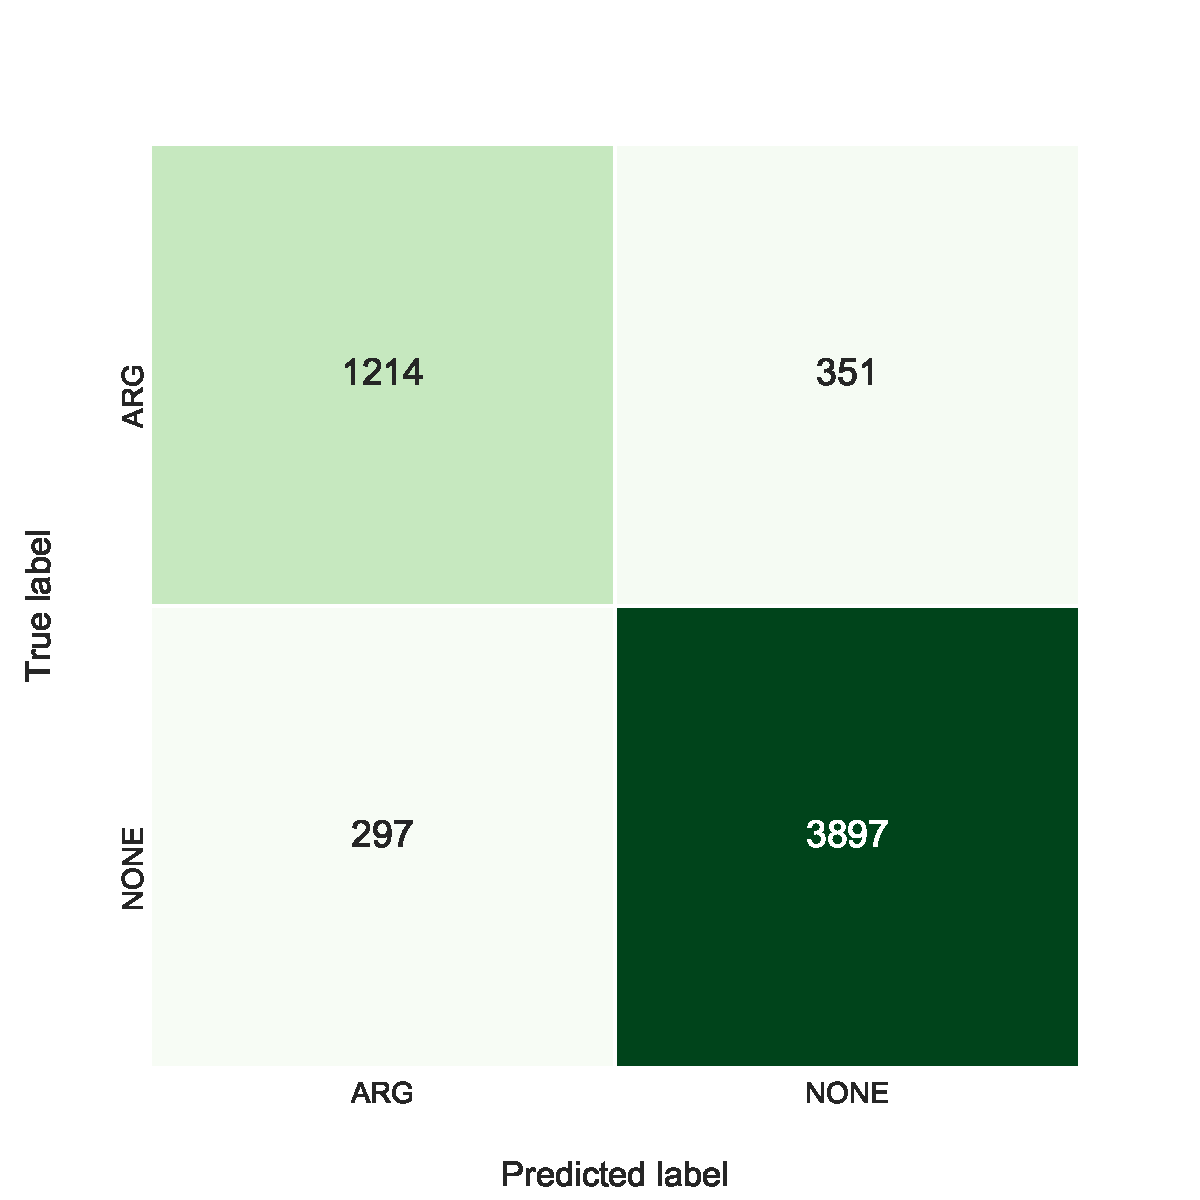
\includegraphics[width=1\textwidth]{images/experiments/conf-InferSent_True}
  \end{minipage} \hfill
    \begin{minipage}{.5\linewidth}
  
     \caption{Confusion matrix for the bag-of-words feature using XGBoost} 
       \label{fig:2_conf_uni}
 \centering
	\includegraphics[width=1\textwidth]{images/experiments/conf-Bag-Of-Words_true}
    \end{minipage} 
\end{figure}
Similar to the three-classes scenario, both feature setups made the same mistakes on 517 sentences. The unigram feature produced 204 unique errors, the sentence embeddings 192. It bears mentioning that 765 of the 913 errors are also present in the three-label scenario, so only 148 errors are new. 


The binary scenario benefits from the reduced class imbalance, yet the errors made are essentially the same. Table \ref{tbl:2_mistakes} shows some example sentences from the 148 new errors.

\begin{table}[h]
\caption{Example sentences for errors made by the classifier in the binary scenario. The objects of interest are printed \textbf{bold}, the assumed error source in \emph{italics}. The class \texttt{ARG} was created by merging the classes \texttt{BETTER} and \texttt{WORSE} before the classification. Confidence shows the confiedence of the annotators and is calculated as \emph{judgments for majority class / total judgments}.}
\label{tbl:2_mistakes}
\begin{tabularx}{\linewidth}{Xrrr}
\toprule
 Sentence & Predicted & Gold & Confidence\\ \midrule
 Why \emph{can't} \textbf{Ford} puts better handling into the FWD Fusion if \textbf{Honda} can do it 10 years ago\emph{?} & \texttt{ARG} & \texttt{NONE} & 0.5\\
 
 \textbf{Java} \emph{isn't} too bad of a first language, but \textbf{Python} is a little easier to pick up. & \texttt{NONE} & \texttt{ARG} & 1 \\
 My minestrone \textbf{soup} is always better \emph{with} homemade \textbf{pasta}. & \texttt{ARG} & \texttt{NONE} & 0.8\\
 
 \textbf{Scala} probably embraces \textbf{Java} \emph{better} than any other language in the book. & \texttt{ARG} & \texttt{NONE} & 0.8 \\
 
 \textbf{Windows 8} has efficiency improvements over \textbf{Windows 7}, making it about \emph{10\% faster} overall. & \texttt{NONE} & \texttt{ARG} & 1 \\
\bottomrule
\end{tabularx}

\end{table}

The first sentence is an example for the problems with questions and, like the second, negations. In fourth and fifth sentence, the cue word appears after the objects.
\FloatBarrier
\section{Discussion}
Section \ref{sec:3_results} only shows the results for the best performing configuration of each feature. This is, for all cases, the middle part of the sentence. Intuitivly, this makes sense. Comparative sentences are often formed after the pattern \emph{Noun Verb Comparative Adjective Noun}, as in \emph{\enquote{Python is better than Ruby}}. Sentences which are not formed after this pattern caused wrong predictions, as presented in \ref{sec:error_analysis}.
 Using the full sentence worked second best. Adding the first and/or last part of the sentence did not increase the f1 score at all, no matter if the same or another represenation type than the one for the middle part is used. The first and second part alone never got an f1 score above the baseline.

Replacing or removing the objects did not increase the score significantly. In most cases, the difference in the f1 score between no replacement/removal and the best replacement/removal strategy was only reflected in the third or fourth decimal place. Hence, the concrete objects are not important at all for the classification. This is also supported by the fact that adding the word vectors of the objects as features did not increase the result for any vector representation. All in all, no combination of vector representations increased the score in any way.

An interesting observation is that the simple bag-of-words model performs almost equal to the more complex models. Even a single boolean feature which captures if the sentence contains a comparative adjective yields an f1 score way over the baseline.

As expected, the smallest class in the data set caused the biggest problems. The recall for \texttt{WORSE} is about three times below the recall for \texttt{BETTER}. Looking at the confusion matrices in figure \ref{fig:3_conf_uni} and \ref{fig:3_conf_inf}, \texttt{WORSE} was confused with \texttt{NONE} for the majority of cases. Intuitivly, a confusion between \texttt{WORSE} and \texttt{BETTER} was expected, since both classes should reflect special cases of a class \texttt{ARG}.

Another interesting obersavtion is that the three-class scenario and the binary scenario made mistakes on the same sentences. In fact, the majority of mistakes made by the binary scenario were made by the three-classes scenario as well.


\section{Evaluation with the held-out data}
tbd
\label{sec:final}

